% #####################################################################################
% Bacheloerarbeit:
% #####################################################################################
% Dokumentformat
\documentclass[12pt, a4paper]{scrreprt}
%\documentclass[12pt, a4paper]{scrreprt}

% Zeichensatz festlegen
\usepackage[utf8]{inputenc} %Linux
% \usepackage[latin1]{inputenc} %Windoof
% \usepackage[T1]{fontenc}
% \usepackage[ngerman]{babel}
\usepackage[english]{babel}

% Damit Text ``gesperrt'' werden kann
\usepackage{soul}

\usepackage{float}

% Paket fuer Grafiken
\usepackage{graphicx}

% Pakete fuer Tabellen
% \usepackage{color,colortbl}
\usepackage{booktabs}

% Paket fuer Kopf und Fusszeilen
\usepackage{fancyhdr}
\pagestyle{fancy}

% remember chapter number and title
\renewcommand{\chaptermark}[1]%
	{\markboth{#1}{}}
\renewcommand{\sectionmark}[1]%
	{\markright{\thesection\ #1}}

% positioning
\lhead[\fancyplain{}{\bfseries\thepage}]%
	{\fancyplain{}{\bfseries\rightmark}}
\rhead[\fancyplain{}{\bfseries\leftmark}]%
	{\fancyplain{}{\bfseries\thepage}}
\cfoot{}

\fancypagestyle{plain}{%

\lhead[\fancyplain{}{\bfseries\thepage}]%
	{\fancyplain{}{}}

\rhead[\fancyplain{}{}]%
	{\fancyplain{}{\bfseries\thepage}}
}

% Einruecken verhindern
\parindent 0pt

% Leerzeile nach Absatz einfuegen
\parskip 12pt

% Zeilenabstaende
\usepackage{setspace}

% Roemische Zahlen
\newcommand{\RM}[1]{\MakeUppercase{\romannumeral #1{}}}

% Bibtex
\usepackage{bibgerm}
%\usepackage{babelbib}

% Abkürzungsverzeichnis
\usepackage[printonlyused]{acronym}

% Bilder nebeneinander, ...auskommentiert wegen \subcaption
\usepackage{subfig}

% Abbildungsverzeichnistiefe einstellen
\captionsetup{lofdepth=4}

% Eurosymbol
\usepackage[right]{eurosym}

% Fussnoten ueber alle kapitel zaehlen
\usepackage{chngcntr}
\counterwithout{footnote}{chapter}

% Listings
% \usepackage{listings}
% \usepackage{xcolor}
% \definecolor{hellgrau}{rgb}{0.9,0.9,0.9}
% \definecolor{colKeys}{rgb}{0,0,1}
% \definecolor{colIdentifier}{rgb}{0,0,0}
% \definecolor{colComments}{rgb}{1,0,0}
% \definecolor{colString}{rgb}{0,0.5,0}
% \lstset{
%     float=hbp,
%      basicstyle=\ttfamily\color{black}\small,
% % %     basicstyle=\ttfamily\color{black}\small\smaller,
%     identifierstyle=\color{colIdentifier},
%     keywordstyle=\color{colKeys},
%     stringstyle=\color{colString},
%     commentstyle=\color{colComments},
%     columns=flexible,
%     tabsize=2,
%     frame=single,
%     extendedchars=true,
%     showspaces=false,
%     showstringspaces=false,
%     numbers=none,
%     numberstyle=\tiny,
%     breaklines=true,
%     backgroundcolor=\color{hellgrau},
%     breakautoindent=true
% }

% Für PDF-Header
\usepackage[
	bookmarks=true,
	bookmarksopen=true,
	bookmarksnumbered=true,
	breaklinks=true,
	colorlinks=true,
	linkcolor=black,
	anchorcolor=black,
	citecolor=black,
	filecolor=black,
	menucolor=black,
	urlcolor=black
]{hyperref}

\hypersetup{
	pdfstartpage=1,
	pdftitle={Bachelorarbeit},
	pdfauthor={Vorname Nachname},
	pdfsubject={Titel der Arbeit},
	pdfkeywords={Bachelorarbeit},
}

% mehrere Literaturverzeichnisse
\usepackage{multibib}

% Definition des citebefehls für Literatur
%\newcites{lit}{Bibliography}
% Definition des citebefehls für Internet
\newcites{int}{Literature}

% ############### Weiteres Zeug für moi #######################
% schöne autotabellen
\usepackage{booktabs}

% Farben! 
\usepackage{xcolor}

% Mathe Zeichen
\usepackage{amsmath}
\usepackage{amssymb}
\newcommand{\R}{\mathbb{R}}

% hyperrefs
\usepackage{hyperref}

% svg 
%\usepackage{svg}

% For subplots in plots?
% \usepackage{subcaption}

% #####################################################################################
% Dokument Beginn
% #####################################################################################
\begin{document}

% Seiten mit roemischen Zahlen beschriften
\pagenumbering{roman}

% Deckblatt
%\null \thispagestyle{empty}

% #####################################################################################
% Titelseite
% #####################################################################################
\begin{titlepage}
	\begin{figure}[ht]
		\centering
		
\includegraphics[width=0.6\textwidth]{images/Logo_UniJena.png}
	\end{figure}	
	\vspace*{1cm}
	\begin{center}
		\bfseries
		\LARGE Political Polarity in US Twitter\\
		\vspace*{3cm}
		\large \so{Seminar BigData}\\
		\vspace*{1cm}
		\normalsize at the \\ Friedrisch Schiller University of Jena\\
		Faculty of Mathematics and Computer Science\\Graduate Degree Computer Science\\
		\vspace*{4cm}
		\begin{tabular*}{\textwidth}[]{p{0.5cm}p{9.5cm}p{10cm}}
			& submitted to				 & submitted by\\
			& Prof. Dr. Bücker,			 & Kenny Gozali,\\
			& Dr. rer. nat. Bosse and	 & Chris Gerlach and\\
			& Herrn Schoder				 & Walter Ehrenberger\\
			\vspace*{2cm}
		\end{tabular*}
		Jena, \today
		\vfill
	\end{center}
\end{titlepage}

% #####################################################################################
% Abstract
% #####################################################################################
\newenvironment{changemargin}[2]{%
\begin{list}{}{%
\setlength{\topsep}{0pt}%
\setlength{\leftmargin}{#1}%
\setlength{\rightmargin}{#2}%
\setlength{\listparindent}{\parindent}%
\setlength{\itemindent}{\parindent}%
\setlength{\parsep}{\parskip}%
}%
\item[]}{\end{list}}

\begin{abstract}

\begin{changemargin}{2cm}{2cm}
  
{\centering \textbf{Abstract} \par}
\medskip

I am not quite sure yet what my topic will be about. Initially i wanted to write about the evolution of the critique on AI. Why would i stop that, there s no real reaseon for it now is there? I should probably read some more before i go further in to this topic, thouuuugh there is another nice paper online that deals with a similar situation.

\end{changemargin}

\end{abstract}

% #####################################################################################
% Inhaltsverzeichnis
% #####################################################################################
\onehalfspacing
%\setcounter{secnumdepth}{4}
\setcounter{tocdepth}{2}
\tableofcontents
\newpage

% #####################################################################################
% Abbildungsverzeichnis
% #####################################################################################
\listoffigures
\newpage

% #####################################################################################
% Abkuerzungsverzeichnis
% #####################################################################################
%\singlespacing

%\chapter*{Abkürzungsverzeichnis}

{
\makeatletter
\renewcommand*{\dotfill}
	{%
		\leavevmode\leaders
		\hbox{$\m@th \mkern \@dotsep mu\hbox{.}\mkern \@dotsep mu$
	}
	\hfill\kern\z@
\makeatother
}

\begin{acronym}[TM]
	\setlength{\itemsep}{-1.1\parsep}
	\acro{RF}{Random Forest}
\end{acronym}

%\newpage

% #####################################################################################
% Inhalt
% #####################################################################################
% Seiten mit `"`normalen"' arabischen Zahlen beschriften
\pagenumbering{arabic}
\onehalfspacing


% #####################################################################################
% Kapitel 1
% #####################################################################################
\chapter{Introduction}
%	\section{Problemstellung}
	Sooome Text

	\begin{figure}[ht]
		\centering
		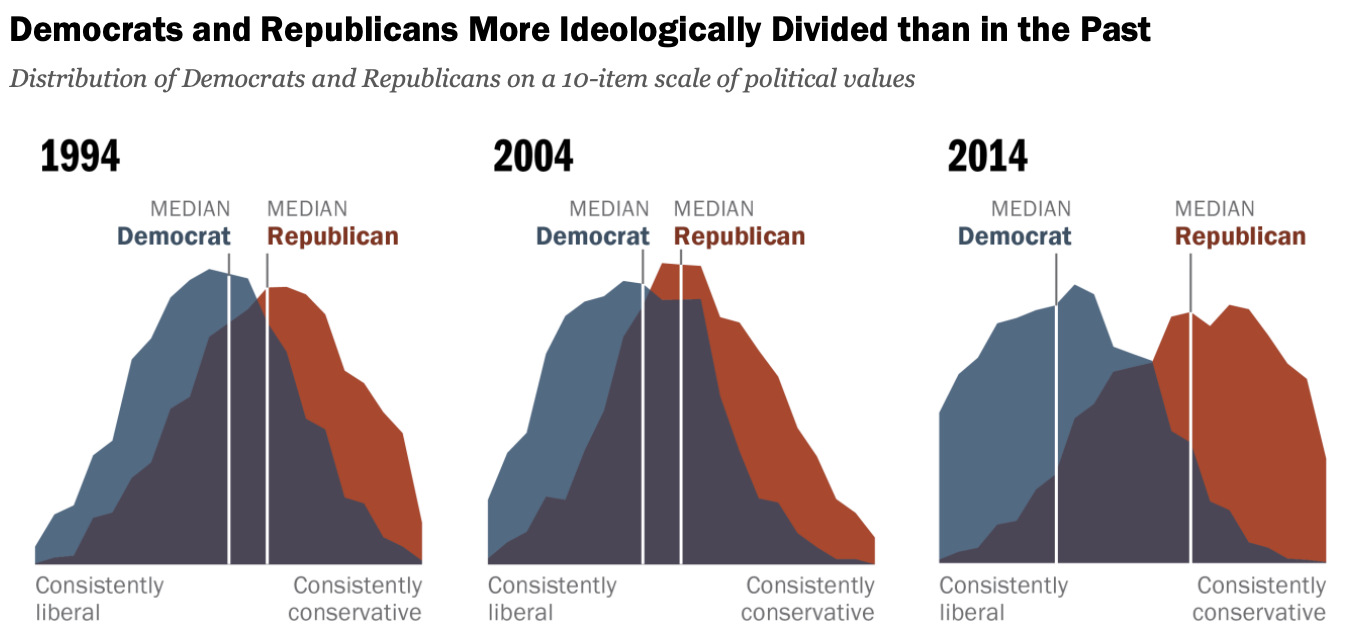
\includegraphics[width=0.9\textwidth]{images/Kapitel1/PoliticalPolarization}
		\captionof{figure}{Greaaaafik}
	\end{figure}
	


Hier kommt der Text hin.

Zitiere \citeint{dartMouth} Internetverzeichnis.

Oder zitiere \citelit{politicalPolarization} Literaturverzeichnis.

	
% #####################################################################################
% Kapitel 2
% #####################################################################################
%\chapter{Getting data (good title missing)}
\chapter{Our project}
	\section{Background}


	In diesem Kapitel sollen die verwenden Bibliotheken und der Grund für ihre Verwendung genauer beleuchtet werden. Damit wir Daten generieren konnten bzw. 
	können, haben wir die Bibliothek GetOldTweets3 verwendet. Mit einer öffentlich zugängliche Userliste für Politiker aus Amerika wurden dann mit diesem 
	Packages die Daten erhoben. Zur Weiterverarbeitung der Daten haben wir NLTK und TextBlob genutzt. Beides sind Tools für die Verarbeitung von Sprache. Um 
	eine Analyse über  die Verarbeiteten Ausgaben durch ein Map-Reduce laufen zu lassen, haben wir als letztes Package Sparks verwendet, um eine zeit 
	effiziente Verarbeitung zu gewährleisten.  
	
	 
	\subsection{GetOldTweets3-Pakage}
	
	GetOldTweets3 ist ein kostenlose Python 3 Packages mit welchen Twitterdaten ohne API-Schlüssel abgerufen werden können.
	Mit GetOldTweets3 können Sie Tweets mit einer Vielzahl von Suchparametern wie Start-/Enddatum, Benutzername(n), Textabfrage 
	und Referenzortbereich durchsuchen. Außerdem können Sie angeben, welche Tweet-Attribute Sie einbeziehen möchten. Einige Attribute
	sind: Nutzername, Tweettext, Datum, Retweets und Hashtags. \citeint{userguid} 
	Die offizielle API von Twitter hat eine lästige Zeiteinschränkung, weshalb man keine Tweets älter als eine Woche abrufen 
	kann. Es gibt einige Tools die Zugang zu älteren Tweets anbieten, diese sind jedoch meistens kostenpflichtig. Das Forscher-
	team hat nach einem andere Tool gesucht die diese Aufgaben übernehmen, wodurch die Wahl auf das Package GetOldTweets3 gefallen 
	ist. \citeint{python}   	
	Die Analyse des Codes von GetOldTweets3 und die Funktionsweise des Searchthrough Browsers von Twitter zeigt wie das Packages auch
	an alte Tweets kommt. Grundsätzlich, wenn sie auf Twitter seiten eingeben oder User suchen, startet ein Scroll-Loader. D.h. wenn sie
	dann weiter nach unten scrollen, bekommen sie immer mehr Tweets zu den Suchbegriffen. Diese ganzen Tweets bekommen sie durch Abfragen 
	an einen JSON-Provider. GetOldTweets3 imitiert den Searchthrough Browser von Twitter um den Scroll-Loader zu starten und zieht sich dann 
	anhand, der Abfragen an einen JSON-Provider die JSON-Datei und gibt diese decodiert zurück um dann alle Twitts anhand der oben gegebenen 
	Parameter herauszufiltern. Dies kann man in Quelle \citeint{github}, dem Github-Repositorium gut nachvollziehen. Somit ist es möglich sowohl 
	aktuelle als auch sehr alte Tweets zu scrapen. \citeint{github}
	
	
	\begin{figure}[ht]
		\centering
		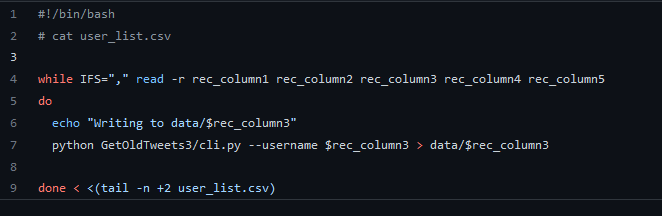
\includegraphics[width=0.9\textwidth]{images/Kapitel2/Code_Beispiel_1}
			\caption{\label{fig:CodeBeispiel}Code Beispiel für das Scrapen der Tweets}{Ist eine Python Bibliothek mit der Twitter Daten durch den Scroll-Loader 
			        des Searchthrough Browsers von Twitter als JSON-Datei abgerufen werden können.}
	\end{figure}
	
	So kann durch eine paar Zeilen Code, wie man in der Abbildung \label{CodeBeispiel} sieht, eine bash-Datei erstellt werden, durch welche die Daten gesucht 
	und abgespeichert werden. Das Scraping an sich kann durch die Größe der JSON-Datei einige Zeit in Anspruch nehmen. Wir haben gerade mal 2 Millionen Tweets 
	insgesamt bei einer Laufzeit von ca. 35 Stunden.  
	

	\subsection{NLTK-Natural language Toolkit}
	
	NLTK ist ein Python Package für die Arbeit mit menschlichen Sprachdaten. Es bietet einfach zu bedienende Schnittstellen zu über 50 Korpora
	und lexikalischen Ressourcen wie WordNet, zusammen mit einer Reihe von Textverarbeitungsbibliotheken für Klassifizierung, Tokenisierung, 
	Stemming, Tagging, Parsing und semantische Schlussfolgerungen, Wrapper für industrielle NLP-Bibliotheken und ein aktives Diskussionsforum. \citeint{nltk} 
	Aus diesem Grund bietet NLTK sehr viele Möglichkeiten zur Vorverarbeitung und Analyse, benötigt aber auch einen gewissen Zeitrahmen zur 
	Einarbeitung in die Analysen. Aus diesen Grund hat sich das Forscherteam dafür entschieden NLTK nur zur Vorverarbeitung zu nutzen und TextBlob
	für die Semantische Analyse zu nutzen. Warum sich für TextBlob entschieden wurde, wird genauer in 2.1.3 besprochen. So verwenden wir den Wordcorbus
	von NLTK für englische Stoppworte, da wir diese nicht mit in unseren Analysen haben wollen. Für eine individuelle und sehr ausführliche semantische Analyse 
	bietet NLTK sehr viele Möglichkeiten, durch die Interaktion mit verschiedenen Packages in Python, was aber den oben genannten Zeitrahmen benötigt, zum 
	einarbeiten. Der Vorteil von NLTK gegenüber TextBlob sind genau diese Interaktionen mit anderen Packages. Für größere Projekte, bei denen man die 
	semantische Analyse auch individuell anpassen möchte,sollte man eher die NLTK Bibliothek benutzen. NLTK ermöglicht es durch verschiedene 
	Vorverarbeitungsschritte, welche in der Bibliothek eingebaut sind eine individuelle Pipeline und Analyse zu erstellen.
	
	\begin{figure}[ht]
		\centering
		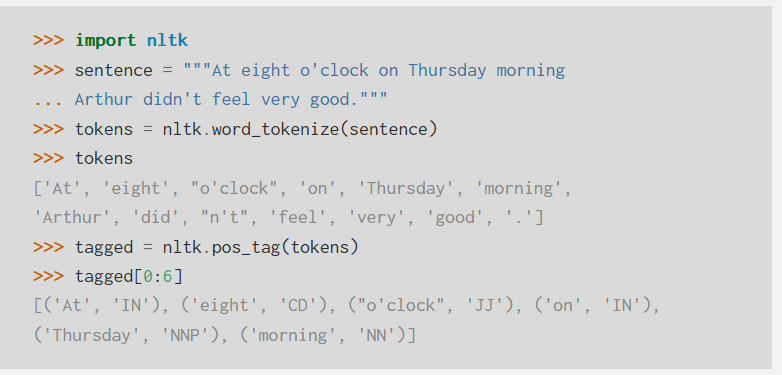
\includegraphics[width=0.9\textwidth]{images/Kapitel2/Code_Beispiel_2}
			\caption{\label{fig:CodeBeispiel}Code Beispiel für das Arbeiten mit NLTK}{Tokenizierung und Tagging von Texten mit NLTK}
	\end{figure}    	
		
	
	
	\subsection{TextBlob}
	
	TextBlob ist eine Python Bibliothek für Python zwei und drei. Diesem Package arbeiten, ähnlich wie NLTK, mit verschiedenen Packages welche in Python schon 
	verfügbar sind. In TextBlob sind zwei verschiedene Semantische Analysen vorhanden. Da gibt es zum einen die Patternanalyse verwendet, welche die Pattern 
	libary in Python von Python nutzt, und dann gibt es da noch die Naive-Bayes-Analyse. \citeint{blob} Hier stellt NLTK zum Beispiel mehr zur Verfügung, aber 
	benötigt damit auch mehr Einarbeitungszeit. Damit bietet TextBlob eine besser Übersicht, weshalb sich das Forscherteam auf Grund der wenigen Zeit für 
	diese Bibliothek entschieden hat. Ein weiter Grund, warum sich schlussendliche für diese Bibliothek entscheiden wurde, ist auch die zwei Outputwerte 
	Polarität und Subjektivität eine gute Anwendungsmöglichkeit für ein Mapreduce darstellen. \citeint{userguideText}	
	In unseren Analysen haben wir die Patternanalyse von TextBlob verwendet, welche uns die Polarität in einem Intervall von [-1, 1] und die Subjektivität im 
	Rahmen von [0, 1] zurück gibt. Ist der Wert bei der Polarität näher an der -1 als an der 1, dann zeigt es einen negative Emotion. Im umgekehrten Fall ist 
	es eine positive Emotion. Bei dem Wert der Subjektivität beschreibt ein Wert der näher an der Null ist eher einen Fakt oder Faktenwissen und je näher er 
	der 1 kommt, desto mehr spielt in die Aussage die eigene subjektive Meinung mit rein. \citeint{semtiment}\citeint{blobkgit}
	Bei der Patternanalyse geht es darum ein Muster bei negativen und positiven Aussagen zu erkennen und dies dann auf neue Testdaten oder unbekannte Daten 
	anzuwenden. Dabei spielt sowohl die Syntax als auch die Semantik und die Wortwahl eine große Rolle. \citeint{pattern}
	Mit etwas mehr Zeit hätte man auch noch die Analyse des Naive-Bayes in einem Mapreduce verwenden können.

	
	\subsection{Sparks}
	
	Sparks ist ein Big Data Framework zur Verarbeitung, Filterung und Analyse von großen Datenmengen. Diese Bibliothek vereinfacht die Anwendung eines 
	Mapreduce, indem es verschiedene Funktionsweisen und Tools dafür anbietet. So begrenzt sich der Programmcode auf die wesentlichen Funktionen eines 
	Mapreduce und verschafft dadurch eine gut Übersicht über den Code. Des weiteren stellt Sparks verschiedene Datenstrukturen zur Verfügung, um die Arbeit mit 
	großen Datenmengen zu erleichtern. Dazu gehört zum Beispiel das Resilient Distributed Datasets (RDD). Ein weiter Vorteil den Sparks bietet ist die hohe 
	Verarbeitungsgeschwindigkeit der Daten.
	Aus diesen Gründen hat sich das Forscherteam entschieden für das Mapreduce, welches in dem Forschungsprojekt Anwendung finden soll, diese Bibliothek zu 
	verwenden.     
	

	

	\section{Data Sanitization}
	
In diesem Kapitel wird näher auf den Programmcode des vorliegenden Forschungsprojektes eingegangen und erklärt, was genau in der Datensammlung und Datenverarbeitung gemacht wurde. Zu Beginn wurden die Daten wie in Punkt \textit{2.1.1 GetOldTweets3} beschrieben, mit der Bibliothek gescrapt und als CSV-Datei abgespeichert. Wie das Scraping in der Bibliothek genau funktioniert, ist ebenfalls unter dem Punkt \textit{2.1.1. GetOldTweets3} beschrieben. Um die gespeicherten Tweets für das MapReduce vor zu verarbeiten, wurden die zur Verfügung stehenden Bibliotheken \textit{NLTK} und \textit{cleantext}.
	
	
	\begin{figure}[ht]
		\centering
		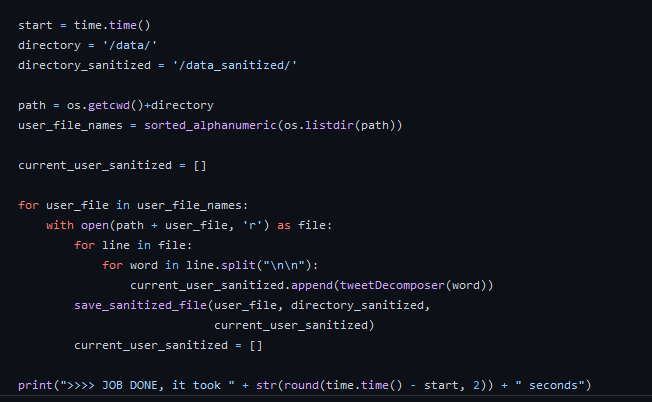
\includegraphics[width=0.9\textwidth]{images/Kapitel2/Code_Datensanierung_1}
		\caption{\label{fig:DataSan}Sanierungs-For-Schleife der Daten}
	\end{figure}
	
Die Variable "directory" und "directory\_ sanitized" geben den Pfad an, in welchem Ordner die Daten gespeichert werden sollen. Mit der Bibliothek \textit{os} von Python können über "os.listdir(pfad)" alle Dateinamen innerhalb dieses Ordners eingelesen werden. Mit der Variable "user\_ file\_ names" wird eine alphanumerisch sortierte Liste der Usernamen der Politiker zurückgegeben, welche dann über eine For-Schleife durchgegangen werden kann, da der Name der CSV-Dateien mit folgendem Muster dem Usernamen entspricht, "Name\_ D" oder "Name\_ R". \textbf{D} steht für demokratisch und \textbf{R} für republikanisch. In dieser Datensanierungsschleife wird die Funktion \textit{tweetDecomposer} verwendet. Diese Funktion übernimmt in der vorliegenden Datensanierung die Hauptaufgabe.
	
%	\begin{figure}[ht]
%		\centering
%		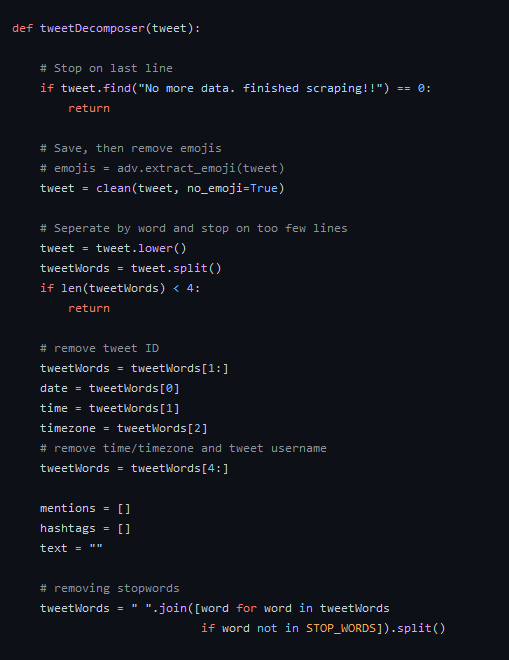
\includegraphics[width=0.9\textwidth]{images/Kapitel2/Code_Datensanierung_2}
%		\caption{\label{fig:DataSanF1}Ausschnitt eins der Sanierungsfunktion der Daten}
%	\end{figure}

Mit der Bibliothek \textit{cleantext} wurden \textit{Emojis} aus dem Text entfernt, wie man in Abbildung ~\ref{fig:DataSanF1} in den ersten Zeilen der Funktion sehen kann. Dann werden alle Worte innerhalb eines Tweets kleingeschrieben und aufgetrennt, damit die ID, die Zeitzone und der Username aus dem Tweet entfernt werden können. Mit \textit{NLTK} werden dann die Stoppworte durch ein \textit{join} aus den Tweets entfernt, sodass man zu den letzten Datensanierungsschritten kommen kann.
	 
%	\begin{figure}[ht]
%		\centering
%		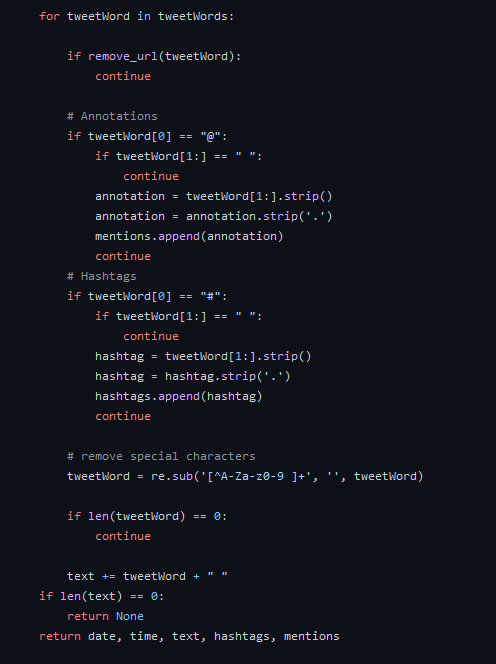
\includegraphics[width=0.9\textwidth]{images/Kapitel2/Code_Datensanierung_3}
%		\caption{\label{fig:DataSanF1}Ausschnitt eins der Sanierungsfunktion der Daten}
%	\end{figure}
	
Da die Annotations und Hashtags gespeichert werden sollen, wurde, wie in Abbildung ~\ref{fig:DataSanF2} zu sehen ist, eine extra For-Schleife eingesetzt. Die For-Schleife läuft über den gesamten Input des Tweets, dazu zählen Datum, Zeit, Username, Hashtag und Emoji. Als Erstes wird überprüft, ob es sich um eine URL handelt oder nicht. Tritt der Fall ein, dass es eine URL ist, wird diese einfach übersprungen und nicht mit abgespeichert. Die Annotations können durch ein "@" erkannt werden, während die Hashtags mit einem "\# " erkannt werden. Beide Erkennungsmarker werden nicht mit abgespeichert. Der restliche Inhalt des Hastags und der Annotation werden in einer extra Liste gespeichert.


Als Letztes wurden alle Sonderzeichen wie Punkte, Kommas und andere Zeichen entfernt. Die Funktion gibt dann alle interessanten Daten für die Analyse zurück. Zum Schluss werden diese Daten in einer CSV-Datei gespeichert. Als nächster Schritt folgt die Hautanalyse unseres Projektes in 2.3.
	\section{MapReduce (good title missing)}

Hallo Palmoooooo und Walta

		
% #####################################################################################
% Kapitel 3
% #####################################################################################
\chapter{Analysing the data}

	\section{data1 (good title missing)}

Hey Kennyyyyy
	\section{data2 (good title missing)}

Hey Kennyyyyy				
		
% #####################################################################################
% Kapitel 4
% #####################################################################################
\chapter{Schluss}

	\section{Resume}

Wie sie sehen sehen sie nichts. 
		
		
% #####################################################################################
% Kapitel 5
% #####################################################################################
%\chapter{Discussion} 
%	It is important to be grounded in the present, not in a metaphorical sense, but by admitting the limits of what current technology is able to provide us with. Even though highly specialized AIs have long surpassed human experts in narrow domains, they fail to generalize and often lack common sense, apart from countless other flaws previously discussed. Arguing that an AI, being better at a task than a human expert shows signs of real intelligence, is like saying wolfram alpha is a better mathematician than most humans.

Even Dreyfus could not have anticipated that AI scientists would realize their mistake, and give in to the valid arguments against symbolism by pursuing different paths. So he claimed that AI was impossible. However AI researchers commited the same fallacy by thinking that such programs were not necessary. Thinking that current approaches if only developed further would result in strong AI. Neither of them were correct. But both of them were necessary to surpass what has been.

Alan Turing once said, \textit{''We cannot so easily convince ourselves of the absence of complete laws of behaviour ... The only way we know of for finding such laws is scientific observation, and we certainly know of no circumstances under which we could say, We have searched enough. There are no such laws.''} \citelit{turing}. Arguing that we can create a mind is the same as arguing there has to be a god, or as arguing there cant be a god. Even though current approaches will certainly not surprise us with the sudden emergence of consciousness, this can not be mapped on the future.

% #####################################################################################
% Anhang
% #####################################################################################
\begin{appendix}
	\chapter{Code Example Sanitization 1}
		%\label{lab:appendix_a}
 		...
 	\chapter{Code Example Sanitization 2}
	 	%\label{lab:appendix_b}
			\begin{figure}[ht]
		\centering
		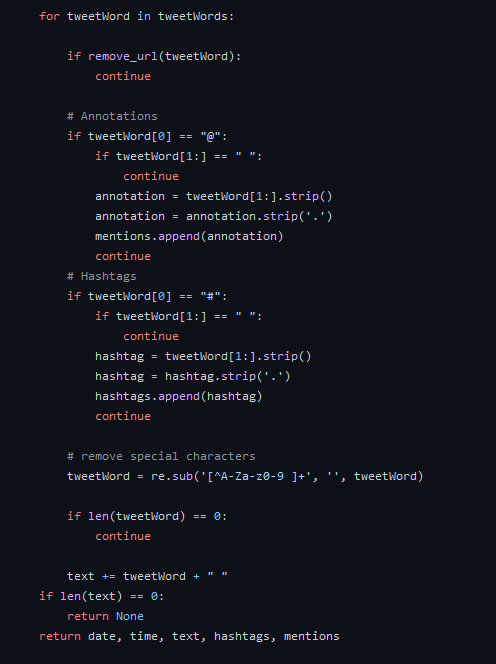
\includegraphics[width=0.73\textwidth]{images/Kapitel2/Code_Datensanierung_3}
		\caption{\label{fig:DataSanF2}Ausschnitt eins der Sanierungsfunktion der Daten}
	\end{figure}
\end{appendix}

% #####################################################################################
% Literaturverzeichnis
% #####################################################################################

% Definitionen von LIT und INT im header, ggf aus oder ein kommentieren.

% Only citations you use are appended to the literature. If you use none of them it will
% throw an error :) Oh and use $ make to build the literature bib!

%\bibliographylit{literature/literature}
%\bibliographystylelit{alphadin}
%\addcontentsline{notoc}{chapter}{Literature Bibliography}
%\newpage

\bibliographyint{literature/internet}
\bibliographystyleint{alphadin}
\addcontentsline{notoc}{chapter}{Literature}
\newpage

% #####################################################################################
% Eidesstattliche Erklaerung
% #####################################################################################
%\chapter*{Declaration}
%% Ich erkläre hiermit, dass ich die vorliegende Arbeit selbständig und ohne Benutzung
% anderer als der angegebenen Hilfsmittel angefertigt habe; die aus fremden Quellen
% direkt oder indirekt übernommenen Gedanken sind als solche kenntlich gemacht.
% Die Arbeit wurde nach meiner besten Kenntnis bisher in gleicher oder ähnlicher Form
% keiner anderen Prüfungsbehörde vorgelegt und auch noch nicht veröffentlicht.\\[6ex]
I hereby declare that the presented paper was written independently and without the usage of 
other than the specified tools; thoughts and ideas directly or indirectly taken from 
foreign sources are marked as such. \\[6ex]

Jena, the \today

\rule[-0.2cm]{5cm}{0.5pt}

\textsc{Surname Lastname}
\thispagestyle{empty}

\end{document}
